\documentclass{article}
\usepackage[T1]{fontenc}
\usepackage[utf8]{inputenc}
\usepackage{lipsum}

\begin{document}

\title{Documento di Test}
\author{GitHub Actions}
\date{\today}

\maketitle

\section{Introduzione}
Questo è un semplice documento di prova per testare la compilazione automatizzata con GitHub Actions.

% TODO: \usepackage{graphicx} required
\begin{figure}
	\centering
	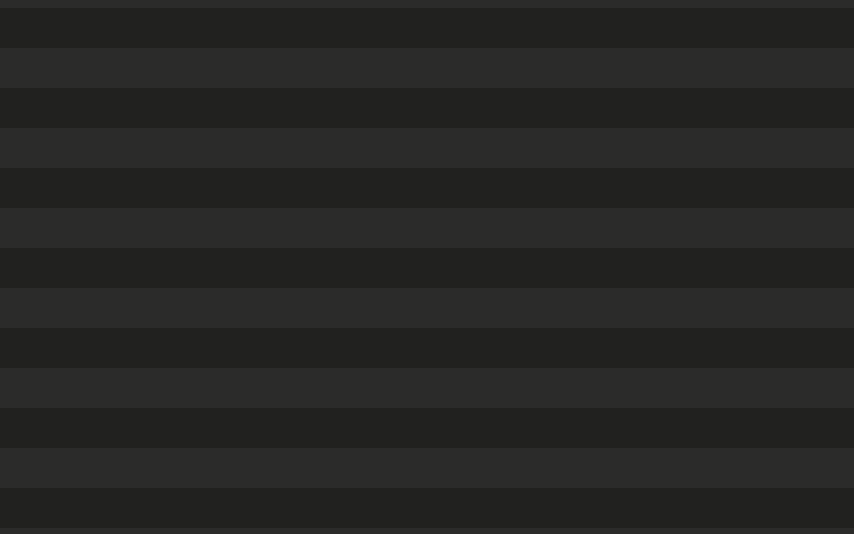
\includegraphics[width=0.7\linewidth]{Immagini/test}
	\caption{}
	\label{fig:test}
\end{figure}


\section{Testo di riempimento}
\lipsum[1-3]

\end{document}
